%% MODELO DE LATEX PARA TRABALHOS ACADÊMICOS

\documentclass[
	% -- opções da classe memoir --
	12pt,				% tamanho da fonte
	% openright,			% capítulos começam em pág ímpar (insere página vazia caso preciso)
    oneside,			% para impressão somente frente. Oposto a twoside (frente e verso)
	a4paper,			% tamanho do papel. 
	% -- opções da classe abntex2 --
	%chapter=TITLE,		% títulos de capítulos convertidos em letras maiúsculas
	%section=TITLE,		% títulos de seções convertidos em letras maiúsculas
	%subsection=TITLE,	% títulos de subseções convertidos em letras maiúsculas
	%subsubsection=TITLE,% títulos de subsubseções convertidos em letras maiúsculas
	% -- opções do pacote babel --
	english,			% idioma adicional para hifenização
	french,				% idioma adicional para hifenização
	spanish,			% idioma adicional para hifenização
	brazil,				% o último idioma é o principal do documento
	]{abntex2}


% ---
% PACOTES
% ---
\usepackage{graphicx}			% Inclusão de gráficos
\graphicspath{{img/}}
% ---
% Pacotes fundamentais 
% ---
\usepackage{cmap}				% Mapear caracteres especiais no PDF
\usepackage{lmodern}			% Usa a fonte Latin Modern
\usepackage[T1]{fontenc}		% Selecao de codigos de fonte.
\usepackage[utf8]{inputenc}		% Codificacao do documento (conversão automática dos acentos)
\usepackage{indentfirst}		% Indenta o primeiro parágrafo de cada seção.
\usepackage{color}				% Controle das cores

\usepackage{epigraph}
\usepackage{multicol}
\usepackage{multirow}
\usepackage{lipsum}				% para geração de dummy text
\usepackage[brazilian,hyperpageref]{backref}	 % Paginas com as citações na bibl
\usepackage[alf]{abntex2cite}	% Citações padrão ABNT
\usepackage{pdflscape}
\usepackage{xspace}

\newcommand\tool[1]{\textsc{#1}\xspace}
\newcommand\SysNut{\tool{SysNut}}

% --- 
% CONFIGURAÇÕES DE PACOTES
% --- 

% ---
% Configurações do pacote backref
% Usado sem a opção hyperpageref de backref
\renewcommand{\backrefpagesname}{Citado na(s) página(s):~}
% Texto padrão antes do número das páginas
\renewcommand{\backref}{}
% Define os textos da citação
\renewcommand*{\backrefalt}[4]{
	\ifcase #1 %
		Nenhuma citação no texto.%
	\or
		Citado na página #2.%
	\else
		Citado #1 vezes nas páginas #2.%
	\fi}%
% ---

% ---
% Informações de dados para CAPA e FOLHA DE ROSTO
% ---
\titulo{\SysNut - Um sistema de auxílio ao Nutricionista}
\autor{Linneu Magno Lopes de Sousa  
	   \\ Orientador: Prof. Dr. Alcemir Rodrigues Santos
   	   \\ Co-orientador: Jonnison Lima Ferreira %Caso Haja
	   }
\local{Picos - PI}
\data{\today}
\instituicao{%
  Universidade Federal do Piauí
  \par
  Campus Senador Heuvídio Nunes de Barros 
  \par
  Bacharelado em Sistemas de Informação}
\tipotrabalho{Monografia}
% O preambulo deve conter o tipo do trabalho, o objetivo, 
% o nome da instituição e a área de concentração 
\preambulo{Trabalho de Conclusão de Curso apresentado ao
Curso de Bacharel em Sistemas de Informação,
Campus Senador Helvídio Nunes de Barros, da
Universidade Federal do Piauí como parte dos
requisitos para obtenção do referido grau.}
% ---

% ---
% Configurações de aparência do PDF final

% alterando o aspecto da cor azul
\definecolor{blue}{RGB}{41,5,195}

% informações do PDF
\makeatletter
\hypersetup{
     	%pagebackref=true,
		pdftitle={\@title}, 
		pdfauthor={\@author},
    	pdfsubject={\imprimirpreambulo},
	    pdfcreator={LaTeX with abnTeX2},
		pdfkeywords={abnt}{latex}{abntex}{abntex2}{relatório técnico}, 
		colorlinks=true,       		% false: boxed links; true: colored links
    	linkcolor=blue,          	% color of internal links
    	citecolor=blue,        		% color of links to bibliography
    	filecolor=magenta,      		% color of file links
		urlcolor=blue,
		bookmarksdepth=4
}
\makeatother
% --- 


% ---
% compila o indice
% ---
\makeindex
% ---







% ----
% Início do documento
% ----
\begin{document}

% Retira espaço extra obsoleto entre as frases.
\frenchspacing 

% ----------------------------------------------------------
% ELEMENTOS PRÉ-TEXTUAIS
% ----------------------------------------------------------
% \pretextual

% ---
% Capa
% ---
\imprimircapa
% ---

% ---
% Folha de rosto
% (o * indica que haverá a ficha bibliográfica)
% ---
\imprimirfolhaderosto*
% ---






% ---
% Agradecimentos
% ---
\begin{agradecimentos}

	Pai Celestial, sou grato eternamente por tua bondade e misericórdia. O Senhor me manteve confiante em busca dos meus sonhos.

	A minha família, agradeço por toda a confiança, apoio e incentivo. Meus pais: Milton José de Sousa e Maria Luzanilda Lopes de Carvalho Sousa, meus irmãos: Ludmilla Moema Lopes de Sousa e Lamarck Mendel Lopes de Sousa. Tenho certeza de que essa conquista não seria possível sem vocês, pois desde o início, foi em quem me espelhei e busquei forças para continuar. Foi também por vocês que busquei essa conquista e que buscarei ainda mais.

	Sou muito grato a minha namorada: Mayara Teresa de Carvalho. Pelo amor, pelo carinho, pelo apoio, inclusive profissional. Você também tornou esse sonho possível. Muito obrigado, meu amor.

	Aos meus mestres, desde o meu primeiro ano na escola até o último período de faculdade. Se existe um profissional que merece ser reconhecido pelo seu trabalho e sua função na sociedade, este precisa ser o professor. Muito obrigado pelo conhecimento compartilhado. Agradeço em especial aos meus orientadores: Ismael de Holanda Leal e Patricia Medyna Lauritzen de Lucena Drumond e meu coorientador Jonnison Lima Ferreira, por dedicarem parte do seu tempo para aperfeiçoar meu trabalho e também tornar essa conquista possível.

	Aos meus amigos, irmãos DeMolay’s e tios maçons. Durante todos esses anos enquanto estive aqui para obter o grau de bacharel em Sistemas de Informação, vocês também fizeram parte do alicerce que me sustentou.

	Eu realmente agradeço a todos que contribuíram direta ou indiretamente para essa conquista. Muito obrigado a todos!


\end{agradecimentos}
% ---

% ---
% Epigrafe
% ---
\vspace*{\fill}
{ \raggedleft
	\textit{Não a nós, Senhor, nenhuma glória para nós, mas sim ao teu nome, por teu amor e por tua fidelidade!. \\
		Salmos 115:1}
	~
}
\pagebreak


% ---
% RESUMO
% ---

% resumo na língua vernácula (obrigatório)
\begin{resumo} %% AQUI COMEÇA A PÁGINA DE RESUMO
 A alimentação é muito importante na vida humana. Devido a vida corriqueira das
pessoas, aumentou-se a demanda pelos \textit{fast-food}, alimentos estes ricos em
substâncias prejudiciais à saúde, causadores das doenças crônicas não transmissíveis. 
A preocupação com a melhora e qualidade de vida faz com que as pessoas busquem cada
vez mais o nutricionista. Por outro lado, o
nutricionista encontra um trabalho que necessita de organização e precisão, do
contrário pode cometer erros que comprometam o seu trabalho com o paciente. Diante
dessas dificuldades, surge a demanda por ferramentas que auxiliem o trabalho do
nutricionista, possibilitando um trabalho com mais agilidade e atenção às
necessidades do seu cotidiano profissional. O sistema deste trabalho propõe uma
ferramenta simples, ao tempo que proporciona uma boa
experiência para o profissional que a utiliza e consequentemente reduz o índice de
obesidade iminente.
 \vspace{\onelineskip}
    
 \noindent
 \textbf{Palavras-chaves}: Alimentação, Sistema de apoio ao
nutricionista, obesidade.
\end{resumo} %AQUI TERMINA A PÁGINA DE RESUMO


\begin{resumo}[Abstract]
Food is very important in human life. Because of people's everyday lives, the demand for fast food has increased. This kind of food is rich in substances harmful to health, chronic non-communicable diseases. The concern with the improvement and quality of life causes people to seek more and more the nutritionist. On the other hand, the nutritionist finds a job that needs organization and accuracy. Inconsequence, he may make mistakes that compromise his work with the patient. Faced with these difficulties, there is a demand for tools that help the nutritionist's job. This work proposal consists of an simple tool and providing a good experience for the professional who uses it and consequently reduces the rate of imminent obesity.
\vspace{\onelineskip}

\noindent
\textbf{Keywords}: Food, Nutritionist support system, obesity.
\end{resumo}


% ---
% inserir lista de ilustrações
% ---

\listoffigures* %% o * indica que não será incluso no sumário
\cleardoublepage %% Pula página
% ---

% ---
% inserir lista de tabelas
% ---

\listoftables*
\cleardoublepage
% ---

% ---
% inserir lista de abreviaturas e siglas
% ---

\begin{siglas}
	\item[DCNT] Doenças Crônicas Não Transmissíveis
 	\item[CSS] \textit{Cascading Style Sheets}
	\item[DRY] \textit{Don’t Repeat yourself}
	\item[ETA] Efeito Térmico dos Alimentos
	\item[GPL] \textit{General Public License}
	\item[HTML] \textit{HyperText Markup Language}
	\item[ITIL] \textit{Information Technology Infrastructure Library}
	\item[JSON] \textit{JavaScript Object Notation}
	\item[MVC] \textit{Model-View-Controller}
	\item[MTV] \textit{Model-Template-View}
	\item[NSF] \textit{National Science Foundation}
	\item[OMG] \textit{Object Management Group}
	\item[ORM] \textit{Object-relational mapper}
	\item[PSF] \textit{Python Software Foundation}
	\item[SGBD] Sistema de Gerenciamento de Banco de Dados
	\item[SP] \textit{Story points}
	\item[SQL] \textit{Structured Query Language}
	\item[TACO] Tabela Brasileira de Composição de Alimentos
	\item[TMB] Taxa Metabólica Basal
	\item[GET] Gasto Energético Total
	\item[URL] \textit{Uniform Resource Locator}
	\item[UML] \textit{Unified Modeling Language}
	\item[VBA] \textit{Visual Basic for Applications}
	\item[VN] Valor de negócio
	\item[XML] \textit{Extensible Markup Language}
\end{siglas}
% ---

% ---
% inserir lista de símbolos
% ---
%\begin{simbolos}
%  \item[$ \Gamma $] Letra grega Gama
%  \item[$ \Lambda $] Lambda
%  \item[$ \zeta $] Letra grega minúscula zeta
%  \item[$ \in $] Pertence
%\end{simbolos}
% ---

% ---
% inserir o sumario
% ---

\tableofcontents*

% ---

% ----------------------------------------------------------
% ELEMENTOS TEXTUAIS  (necessário para incluir número nas páginas)
% ----------------------------------------------------------
\textual


% ----------------------------------------------------------
% Introdução
\chapter{Introdução} 

A alimentação é um dos momentos mais importantes na vida das pessoas tanto
por fatores quanto por fatores sociais, culturais e científicos. É
por meio dela que se obtém a energia necessária para desenvolver atividades diárias
e outros nutrientes primordiais a saúde, como vitaminas e minerais. \cite{proenca}.

O Brasil atualmente passa por uma etapa de transição na alimentação de sua
população, a mesma que antes enfrentava a desnutrição, nos dias atuais apresenta
alta prevalência de obesos, isso pode ser explicado pela mudança drástica na
alimentação. Com o aumento da renda básica das famílias, o \textit{fast-food} tornou-se
presente nas mesas da população brasileira. Alimentos como estes, são ricos em
gordura saturada, açúcar e sódio, os quais são precursores de diversas doenças crônicas não
transmissíveis (DCNT) como, diabetes mellitus tipo II, doenças no sistema
cardiovascular, obesidade mórbida, entre outras \cite{schuster}.
A preocupação com a alimentação e qualidade de vida se faz cada
dia mais presente no cotidiano de todos os brasileiros, decorrência do uso exacerbado
dos \textit{fast-food}. O nutricionista, 
profissional responsável pela prescrição dietoterápica, tem ganho mais cada vez mais espaço no mercado de
trabalho, perante sua importância para manutenção da saúde do ser humano
\cite{brasil}.

Diante da importância do seu trabalho, o nutricionista tem buscado melhorias
no seu atendimento, que por vezes torna-se cansativo perante a vasta quantidade de
cálculos para análise do estado nutricional do paciente, das necessidades energéticas
e para adequação do cardápio. A necessidade de agilizar e aprimorar o atendimento
nutricional acarretou o surgimento de softwares que atendessem as necessidades
básicas como resolução de equações e maior organização dos dados dos pacientes
\cite{vieira}.

A ferramenta proposta neste trabalho, além de ajudar o nutricionista em seu cotidiano de trabalho,
também contribui com a redução do índice de obesidade existente no Brasil, através da utilização da mesma
de forma totalmente gratuita por parte de profissionais da nutrição que acabaram de ingressar no mercado
de trabalho e ainda não possuem nenhuma ferramenta que auxiliem a sua rotina.


\section{Contexto e Problema}

Durante o acompanhamento do paciente, o nutricionista muitas vezes precisa
consultar diversos autores para efetuar um trabalho com mais precisão. Esta etapa do trabalho do profissional
torna-se bastante dificultoso sem o auxílio de uma ferramenta que faça a pesquisa e efetue os cálculos automaticamente.

Para \citeonline{araujo}, antropometria ou avaliação antropométrica é um importante método para avaliação do estado nutricional de um indivíduo e possibilita a detecção de alteração do estado nutricional do mesmo ou até mesmo de coletividades. A Organização Mundial da Saúde (OMS) afirmou em 1995 que a avaliação antropométrica é uma importante ferramenta para detecção para grupos, mas que não deve ser utilizada para diagnóstico final \cite{oms}.

O acompanhamento nutricional individualizado é extremamente importante para
o paciente obter resultados relevantes de acordo com o objetivo traçado pelo
nutricionista, visto que, cada indivíduo possui uma necessidade energética diferente
e a distribuição dos macronutrientes e micronutrientes é realizada de acordo com seu
tipo de organismo, objetivo a ser alcançado e estado nutricional, mediante avaliação
antropométrica.
O nutricionista necessita usar diversas fórmulas
e equações no seu dia a dia, seja para avaliar o estado nutricional do
paciente ou para esquematizar um plano alimentar, fórmulas essas que nem sempre
são sinônimos de praticidade e simplicidade. Esse fator pode trazer perdas
significativas ao profissional da nutrição, visto que são necessários vários cálculos
para prestar atendimento adequado ao seu público-alvo.

Diante disso, é imprescindível uma ferramenta computacional que possibilite a inclusão de refeições, troca de mensagens entre
os usuários do sistema (paciente e nutricionista), 
cálculo das necessidades energéticas e analise do
cardápio auxiliando o profissional durante seu atendimento, trazendo mais
comodidade e rapidez ao seu serviço prestado, de qualquer dispositivo que esteja acessando, desde
que tenha acesso à internet.

\section{Objetivos}

Esse trabalho teve como objeto o desenvolvimento de um sistema para
nutricionistas, voltado para o atendimento nutricional de seus pacientes, atendendo
todas as necessidades primárias de um atendimento individualizado.

\section{Organização do trabalho}
Este trabalho está organizado da seguinte maneira:

{\color{red}

 \begin{itemize}

	\item Capítulo \ref{ch:referencial}  - Descreve descritas todas as ferramentas e técnicas que foram utilizadas durante o desenvolvimento do sistema.
	\item Capítulo 3 – Discute alguns dos trabalhos encontrados que possuem relação com o trabalho do autor.
	\item Capítulo 4 – Explica como o sistema foi implementado e relaciona os casos de uso.
	\item Capítulo 5 – Apresenta e discute os resultados da implementação do projeto.
	\item Capítulo 6 - Aborda os principais achados previstos pelo autor.

\end{itemize}
}
% ---
% referencial teórico
\chapter{Referencial Teórico} \label{ch:referencial}

{\color{red}
Este capítulo apresenta o referencial teórico utilizado para construção dos sistema \textit{Web} proposto (\SysNut). Vale ressaltar que somente os conceitos técnicos referentes à área de Nutrição são apresentados aqui. Detalhes sobre a implementação e ferramentas utilizadas serão apresentados no Capítulo \ref{ch:sysnut}.
}

\section{Atividades do Nutricionista Apoiadas Pelo \SysNut}

{\color{red}
\subsection{Avaliação X}
\subsection{Avaliação Y}
\subsection{Acompanhamento Z}

\section{Conceitos Importantes}

Esta seção aprenta conceitos importantes existentes no contexto das atividades apresentadas na seção anterior\ldots
}


\subsection{Taxa Metabólica Basal (TMB)}

A taxa metabólica basal (TMB) é a quantidade de energia necessária para a
conservação das funções vitais do organismo, representando a maior parte do
consumo energético diário em humanos (cerca de 50\% a 70\%). Sendo calculada em
condições padrão de jejum, repouso físico e mental em ambiente calmo com controle
de temperatura, iluminação e barulhos \cite{ruiz} \cite{harris1}.

A TMB sofre grande influência da massa magra, sexo, idade, composição
corporal e predisposição genética. Fatores como o funcionamento do sistema nervoso
e os hormônios tireoidianos, também contribuem para diferença da TMB entre os
indivíduos. Para a estimativa da TMB, foram desenvolvidas várias equações
matemáticas, utilizando variáveis de fácil mensuração e de baixo custo, como idade,
altura e massa corporal total. Entre tantas equações, são utilizadas as seguintes:
\citeonline{harris1}, sua reformulação \citeonline{harris2} e \citeonline{cunningham} por possuírem grande
aceitabilidade e credibilidade pelas entidades relacionadas a Nutrição \cite{weijs}.

A Taxa Metabólica Basal torna-se indispensável durante o atendimento nutricional, visto
que ele é responsável pela individualização da sua dieta, de forma que possa atender
todas as necessidades calóricas do mesmo, auxiliando na melhora do quadro
nutricional do paciente \cite{pedrosa}.

A ferramenta criada a partir deste trabalho deve então focar nos dados que estas fórmulas podem apresentar
como resultado, a fim de que possa facilitar o atendimento por parte do nutricionista,
ao tempo que o paciente obtenha um resultado com maior satisfação.


\subsection{Gasto Enérgico Total (GET)}

O gasto energético total (GET) compreende a soma de todos os gastos energéticos diários a seguir: A
taxa metabólica basal (TMB) que compreende o gasto energético necessário para a
consumação das funções vitais do organismo; o gasto energético da atividade física
ou fator de atividade (FA), que representa o gasto calórico com as atividades físicas
do cotidiano e o exercício físico; e o efeito térmico dos alimentos (ETA), relacionado
com a digestão, a absorção e o metabolismo dos alimentos. Em indivíduos saudáveis,
a TMB corresponde aproximadamente de 60\% a 70\% do gasto diário, o ETA entre 5\% 
e 15\% e o GEAF ou FA de 15\% a 30\%, sendo este último o elemento que mais varia
entre os indivíduos \cite{hill}. 

\subsection{TACO - Tabela Brasileira de Composição de Alimentos}

Reconhecida oficialmente pelo Ministério da Saúde e produzida pela Universidade de Campinas, o objetivo da TACO é gerar dados sobre a composição dos principais alimentos consumidos no Brasil, de maneira que possa assegurar a confiabilidade dos resultados \cite{taco}. 
Para desenvolver o sistema, foi necessário utilizar-se de um banco de dados que dispusesse das informações nutricionais necessárias para fazer a anamnese alimentar. Para isto, esta ferramenta foi escolhida. A tabela possui mais de 1000 alimentos cadastrados e informa detalhadamente a composição de cada alimento.

% ---
% sysnut
\chapter{\tool{SysNut}: Um Sistema de Auxílio ao Nutricionista} \label{ch:sysnut}


{\color{red} Este capítulo apresenta o que é o \SysNut (Section \ref{sec:sysnut}), bem como \ldots, Feramentas utilizadas na contrução do sistema (Section \ref{sec:ferramental}), \ldots}  



\section{O que é o \SysNut?} \label{sec:sysnut}

\SysNut é um sistema Web que tem o propósito de apoiar as atividades do Nutriciionista. Mais especificamente, o sistema provê suporte para as seguintes atividades:

\begin{itemize}

\item auxilia nos cálculos da rotina de atendimento do paciente;
\item auxilia no agendamento de consultas;
\item {\color{red}tempo em que pudesse visualizar o progresso do paciente. Além disso, foi solicitado a possibilidade de adicionar cardápios as suas consultas para que o paciente possa seguir
suas recomendações.}

\end{itemize}
\ldots 



\section{Implementação das Rotinas do Nutricionista}

Durante todo o desenvolvimento, foi necessário conhecer e entender os
procedimentos de todas as partes (nutricionista e paciente), desde sua primeira visita
ao consultório até o acompanhamento do nutricionista com prescrição cardápio, para
que fosse possível atender às necessidades descritas para que os resultados
fossem mais claros e objetivos.

O sistema foi desenvolvido utilizando a metodologia Scrum (Seção 2.3.1), sem nenhum custo adicional
para os profissionais interessados, onde as análises são feitas sobre as histórias de usuário, sendo que cada uma delas
representa uma necessidade do usuário do sistema. Primeiramente, foi definido o
\textit{Product BackLog}, com as histórias de usuário relatadas pelo \textit{Product Owner}.

%Tabela 1
\begin{figure} [hbt] 
\begin{center}
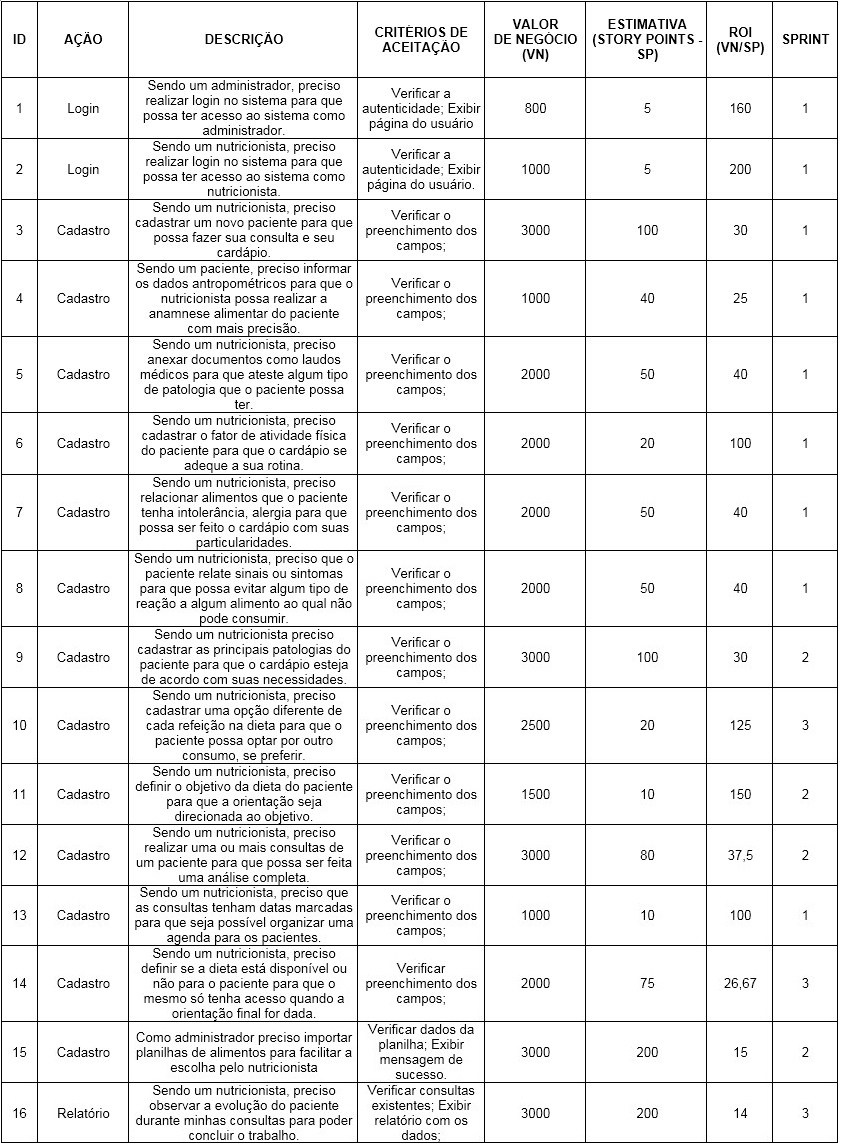
\includegraphics[width=0.90\textwidth]{table.jpg}
\end{center}
\label{table1} 
\caption{\textit{Product BackLog}}
\end{figure}

O \textit{Product BackLog} possui oito atributos, especificados na Figura 4: %colocar tabela

\begin{enumerate}

\item \textbf{ID}: identifica unicamente uma história do \textit{Product BackLog}.
\item \textbf{Ação}: define onde deve ser executado a história.
\item \textbf{Descrição}: contém a história de usuário
\item \textbf{Critérios de aceitação}: contém os critérios para que a ação possa ser
executada com êxito.
\item \textbf{Valor de Negócio}: define a importância da história.
\item \textbf{Estimativa (\textit{Story Points})}: estima o custo do (na visão do desenvolvedor)
para se implementar a história.
\item \textbf{ROI (VN/SP)}: retorno do investimento em relação ao custo.
\item \textbf{\textit{Sprint}}: define em que \textit{Sprint} a funcionalidade foi implementada.

\end{enumerate}

\section{Casos de Uso}

Com base nas histórias elencadas no \textit{Product BackLog}, o sistema foi divido em 2
subsistemas. O primeiro define as ações do administrador e do nutricionista. A Figura 5
mostra o diagrama de casos de uso.

\begin{figure} [hbt] 
\begin{center}
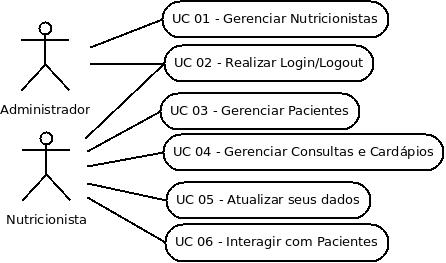
\includegraphics[width=0.9\textwidth]{uc1.jpeg}
\end{center}
\label{uc1} 
\caption{Casos de Uso Administrador e Nutricionista}
\end{figure}

\begin{itemize}
\item \textbf{UC01 – Gerenciar Nutricionistas}

\textbf{- Ator:} Administrador

\textbf{- Descrição:} O usuário administrador pode cadastrar, excluir e
editar os nutricionistas do sistema.

\item \textbf{UC02 – Realizar login e logout}

\textbf{- Ator:} Administrador e Nutricionista

\textbf{- Descrição:} Todos os usuários devem se autenticar, para que o
sistema os identifique e defina suas permissões de acesso.

\item \textbf{UC03 – Gerenciar Pacientes}

\textbf{- Ator:} Nutricionista

\textbf{- Descrição:} O nutricionista pode cadastrar, editar e excluir
pacientes do sistema.

\item \textbf{UC04 – Gerenciar Consultas/Cardápios}

\textbf{- Ator:} Nutricionista

\textbf{- Descrição:} O nutricionista pode cadastrar, editar e excluir
consultas e cardápios feitas sobre um paciente conforme acompanhamento.

\item \textbf{UC05 – Atualizar seus dados}

\textbf{- Ator:} Nutricionista

\textbf{- Descrição:} O nutricionista pode editar dados a seu respeito,
como Nome, E-mail, Senha de Login, etc.

\item \textbf{UC06 – Interagir com Pacientes}

\textbf{- Ator:} Nutricionista

\textbf{- Descrição:} O nutricionista poderá interagir com o paciente através de troca de mensagens pelo próprio sistema.

\end{itemize}

O segundo subsistema, deixa claro as ações do nutricionista em relação ao
paciente. A Figura 6 mostra o diagrama de casos de uso desse subsistema.

\begin{figure} [hbt] 
\begin{center}
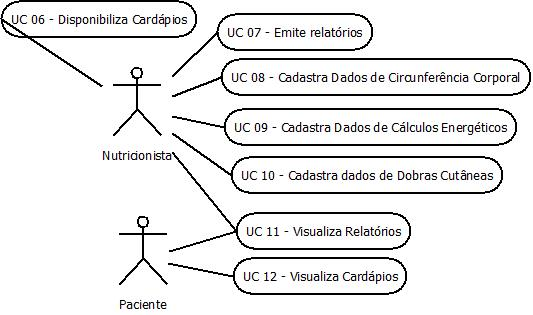
\includegraphics[width=1\textwidth]{uc2.jpeg}
\end{center}
\label{uc2} 
\caption{Casos de Uso Nutricionista e Paciente}
\end{figure}

O diagrama da Figura 6 visa deixar claro as principais ações do nutricionista
em relação ao paciente e o que o paciente pode fazer. Abaixo, segue a descrição
detalhada de cada caso de uso:

\begin{itemize}
\item \textbf{UC07 – Gerenciar Cardápio conforme feedback do paciente}

\textbf{- Ator:} Nutricionista

\textbf{- Descrição:} Uma vez que foi feita a consulta, o nutricionista poderá cadastrar cardápios e fazer alterações do mesmo conforme feedback do paciente.

\item \textbf{UC08 – Emitir relatórios}

\textbf{- Ator:} Nutricionista

\textbf{- Descrição:} O nutricionista é capaz de emitir e disponibilizar
relatórios ao paciente.

\item \textbf{UC09 – Cadastrar Dados de Circunferência Corporal, Cálculos Energéticos, Dobras Cutâneas, Diâmetro Ósseo e Bioimpedância}

\textbf{- Ator:} Nutricionista

\textbf{- Descrição:} O nutricionista poderá cadastrar dados de mensuração sobre o paciente durante a consulta e a partir deles acompanhar seu progresso.

\item \textbf{UC10 – Cadastrar dados de alergia, medicamentos e intolerâncias}

\textbf{- Ator:} Nutricionista

\textbf{- Descrição:} O nutricionista poderá salvar dados acerca de patologias que o paciente possui e medicamentos que ele usa ou possa vir a usar.

\item \textbf{UC11 – Acompanhar o Paciente através de troca de mensagens}

\textbf{- Ator:} Nutricionista

\textbf{- Descrição:} O nutricionista poderá acompanhar o progresso do paciente através de troca de mensagens e por meio delas receber \textit{feedback}.

\item \textbf{UC12 – Visualizar Relatórios e Cardápios}

\textbf{- Atores:} Nutricionista e Paciente

\textbf{- Descrição:} O nutricionista e seu paciente poderão visualizar cardápios e relatórios assim que forem salvos pelo próprio nutricionista.

\item \textbf{UC13 – Interagir com o Nutricionista}

\textbf{- Atores:} Paciente

\textbf{- Descrição:} O paciente poderá interagir com o nutricionista por meio de mensagens e através delas sugerir alterações no cardápio.

\item \textbf{UC14 – Atualizar seus dados}

\textbf{- Atores:} Paciente

\textbf{- Descrição:} O paciente poderá alterar seus próprios dados como login e senha, nome e sobrenome, entre outros.

\end{itemize}

A Figura 7, relaciona as classes do sistema e seus respectivos campos.

\begin{figure} [hbt] 
\begin{center}
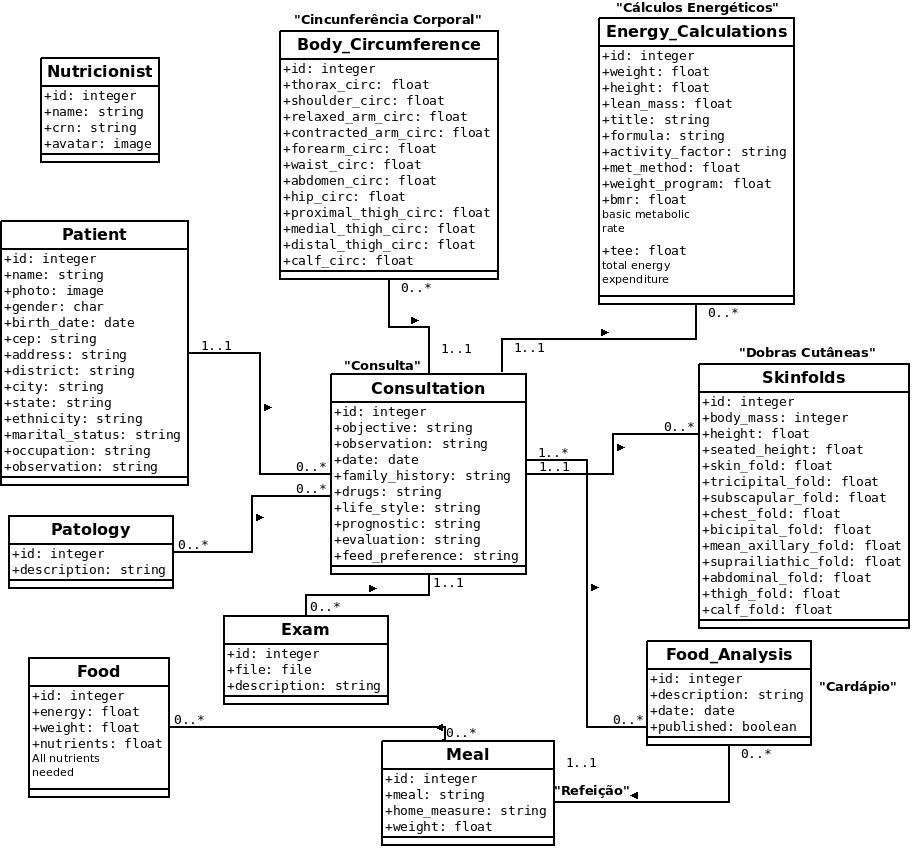
\includegraphics[width=1\textwidth]{bd-sistema.jpeg}
\end{center}
\label{diagClass1} 
\caption{Diagrama de Classes do Sistema}
\end{figure}

O nutricionista é quem cadastra novos pacientes. O paciente possui dados como
dobras cutâneas, circunferência corporal e dados para cálculos energéticos. O
paciente também pode possuir patologias, onde estas podem interferir na sua
alimentação. Além disso, poderá ser cadastrado exames feitos sobre um paciente e
orientações sobre um determinado cardápio. 

Dados como etnia, profissão podem influenciar no fator de atividade física e portanto,
enfatiza-se a presença destes no diagrama da Figura 7. É possível cadastrar cada um destes
dados durante a consulta do paciente. Após feita a consulta, o nutricionista poderá
cadastrar cardápios e consequentemente os alimentos a serem consumidos em cada refeição.
Durante o cadastro de um novo cardápio, o nutricionista seleciona o alimento,
o horário em que será consumido, a quantidade normal, a medida caseira e se este
será publicado ou não, podendo ser editado posteriormente.

Cada alimento, possui micro e macro nutrientes como energia, carboidratos,
lipídios, entre outros. Estes devem ser previamente cadastrados antes de prescrever o
cardápio.

\section{Telas do sistema}

Nesta seção, são apresentadas telas, obtidas durante a implementação do sistema.

\begin{figure} [hbt] 
\begin{center}
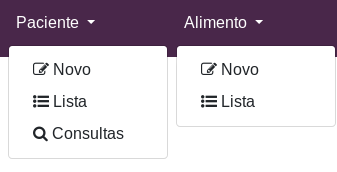
\includegraphics[width=0.55\textwidth]{menuNut1.png}
\end{center}
\label{menuNut} 
\caption{Menu do Nutricionista}
\end{figure}

\begin{figure} [hbt] 
\begin{center}
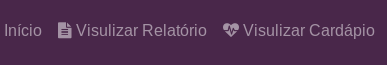
\includegraphics[width=0.55\textwidth]{menuPac1.png}
\end{center}
\label{menuPac} 
\caption{Menu do Paciente}
\end{figure}

É possível observar nas Figuras 8 e 9 que ambos (paciente e nutricionista) podem ter acesso as suas funcionalidades que ficam localizadas na barra superior do navegador.
A Figura 8 mostra todas as funcionalidades do Nutricionista. O Nutricionista
ainda pode emitir relatórios a partir da lista de pacientes acessível no menu. Cada
funcionalidade dessa fica disponível a partir do momento que o Nutricionista realiza 
Login no sistema. A Figura 9 mostra o menu do Paciente. O paciente pode obter dados
do relatório ou do cardápio apenas digitando seu ID e senha do sistema.
Como já mencionado anteriormente, o \textit{Django} possui um sistema de URL's e é através dele que
é feito o tratamento de permissões, uma vez que somente o nutricionista é autorizado de fazer cadastro
de pacientes. A Figura 10 mostra um exemplo de lista de usuários previamente cadastrados no sistema.

\begin{figure} [hbt]
\begin{center}
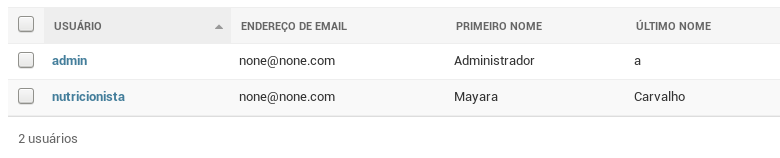
\includegraphics[width=0.55\textwidth]{listaUsuarios.png}
\end{center}
\label{listUser} 
\caption{Lista de Usuários Cadastrados}
\end{figure}

A Figura 11 mostra a tela de cadastro de pacientes, onde é possível cadastrar
seus dados pessoais e os demais dados para fins de acompanhamento do paciente. 

\begin{figure} [hbt]
\begin{center}
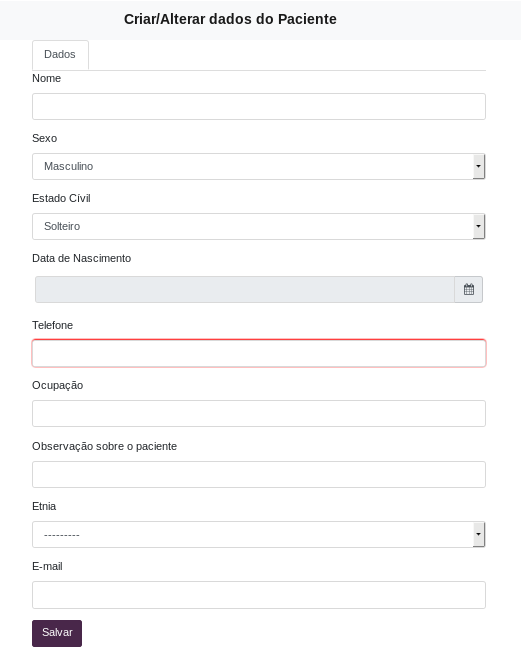
\includegraphics[width=0.55\textwidth]{cadastroPac1.png}
\end{center}
\label{cadastroPac} 
\caption{Tela de Cadastro de Pacientes}
\end{figure}

\begin{figure} [hbt]
\begin{center}
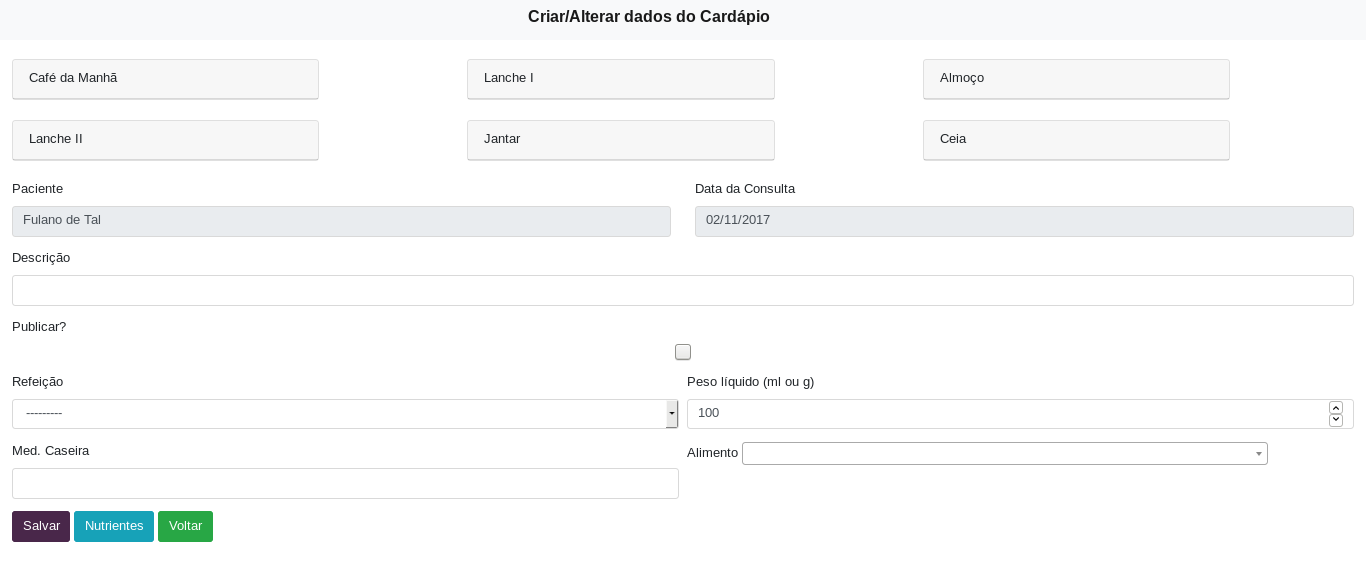
\includegraphics[width=0.55\textwidth]{cadastroCard.png}
\end{center}
\label{cadastroCard} 
\caption{Tela de Cadastro de Cardápio}
\end{figure}

\begin{figure} [hbt]
\begin{center}
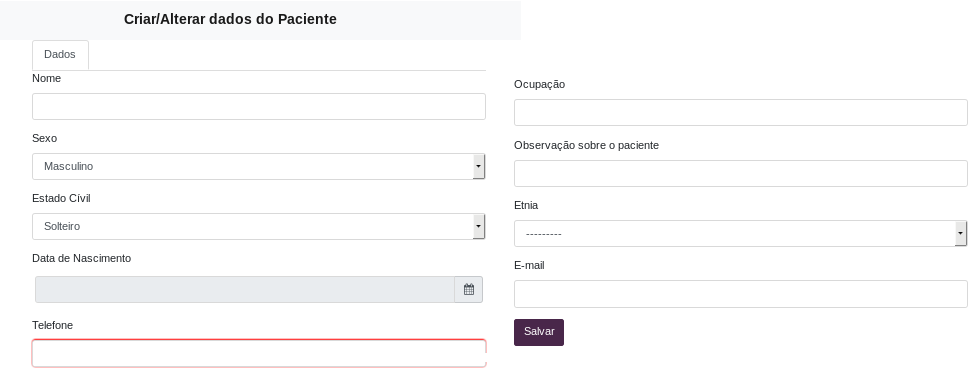
\includegraphics[width=0.55\textwidth]{cadastroCons1.png}
\end{center}
\label{cadastroCons} 
\caption{Tela de Cadastro de Consulta}
\end{figure}

As Figuras 12 e 13 mostram as telas de cadastro de cardápio e consulta,
respectivamente. É durante a consulta que o nutricionista cadastra os dados de
acompanhamento do paciente. O cardápio só poderá ser cadastrado se a consulta já
tiver sido cadastrada previamente.

No cadastro de consultas, o nutricionista cadastra informações de histórico
familiar do paciente, patologias, fármacos que utiliza, além de dados de
acompanhamento como dobras cutâneas, circunferência corporal, entre outros.

O cadastro de cardápio consta dados do paciente, como nome completo e data
em que a consulta foi realizada. Em seguida, a descrição do cardápio, disponibilidade
e os alimentos a serem cadastrados, que devem ter horário de consumo, quantidade
e medida caseira.

\begin{figure} [hbt]
\label{relatPac} 
\caption{Relatório do Paciente}
\begin{center}
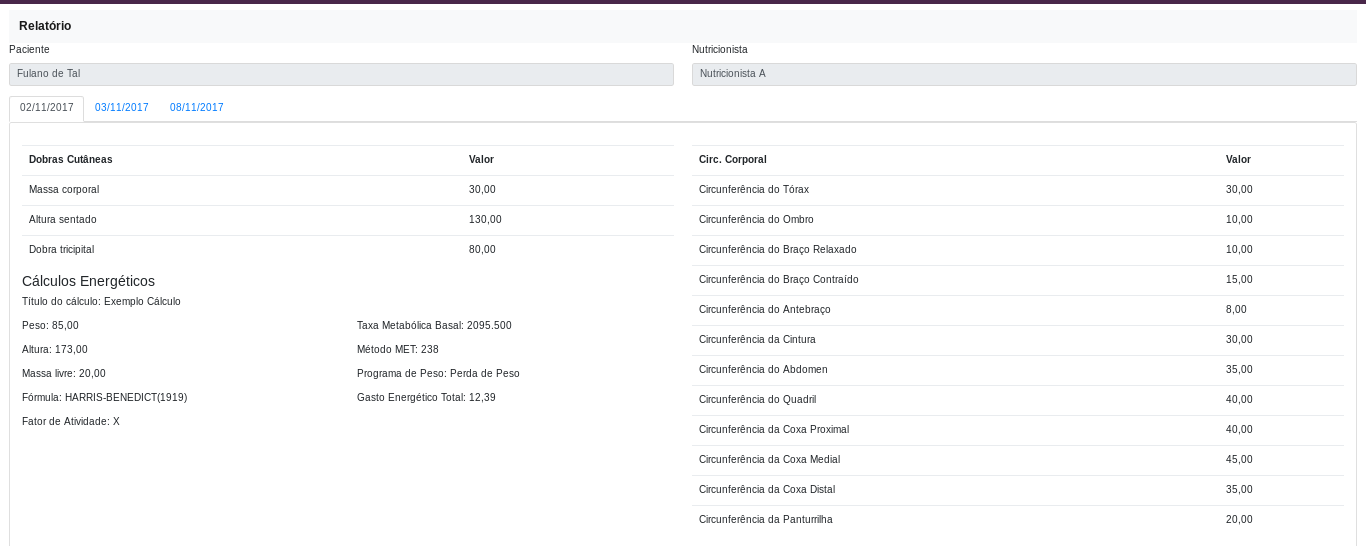
\includegraphics[width=0.75\textwidth]{relatPac1.png}
\end{center}
\end{figure}

A Figura 14 mostra o relatório do paciente, onde é possível ver todos os dados
durante as consultas que foram realizadas e os dados de acompanhamento que foram
obtidos em cada uma delas.

A Figura 15 mostra o cardápio com a descrição e todas as suas informações
nutricionais (macro e micro nutrientes), além do nome do paciente para quem foi
prescrito.
Todas as funcionalidades aqui apresentadas, atualmente, encontram-se
implementadas e já estão prontas para serem usufruidas pelos profissionais interessados.

\begin{figure} [hbt]
\begin{center}
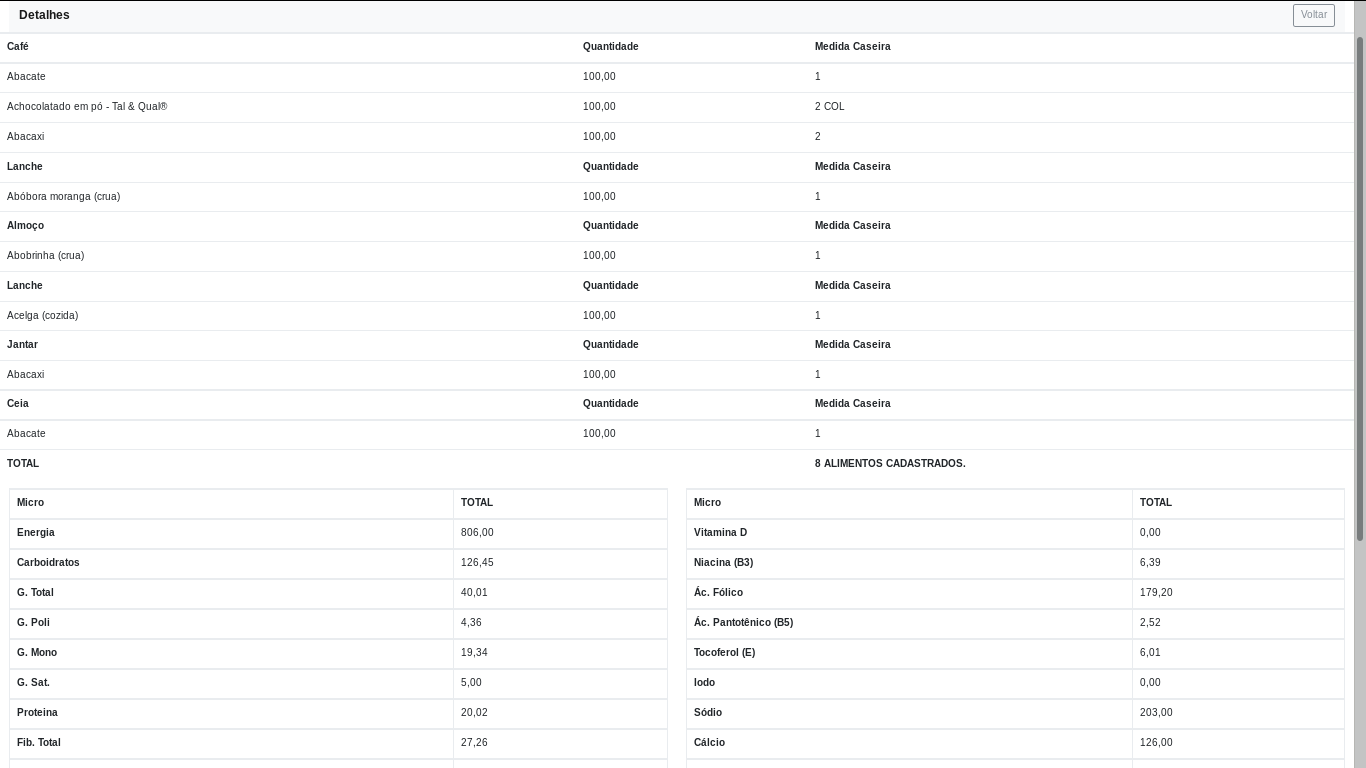
\includegraphics[width=1.0\textwidth]{cardPac1.png}
\end{center}
\label{cardPac} 
\caption{Cardápio do Paciente}
\end{figure}


\section{Ferramentas Utilizadas} \label{sec:ferramental}

Esta seção apresenta os conceitos utilizados durante o desenvolvimento do projeto. \citeonline{tenorio} ressalta a importância da organização e compreensão das informações de um sistema \textit{Web} por parte do usuário, atendendo às necessidades e exigências do mesmo durante o desenvolvimento do sistema.


% --- Seção dentro do capítulo
\subsection{Desenvolvimento \textit{Backend}}
% ---

O lado servidor é onde deve funcionar a lógica principal da aplicação. Todas as
ações são tratadas como requisição. Quando o usuário faz a requisição ao servidor,
é chamado de HTTP \textit{request}. Quando a resposta é enviada pelo servidor, esta ação
é chamada de HTTP \textit{response}.

Os sistemas \textit{Web} funcionam da seguinte maneira: o usuário (cliente) faz uma
requisição de uma página para o servidor e retorna uma resposta para ele através do
navegador. A resposta é interpretada pelo navegador e entregue pelo servidor para o
usuário \cite{niederauer}.

\subsubsection{Python}

Python é uma linguagem de programação de altíssimo nível, orientada a objeto
e de tipagem dinâmica e forte, interpretada e interativa. O nome Python foi dado por
Guido van Rossum do programa da TV Britânica \textit{Monty Python’s Flying Circus} e a
linguagem foi criada por ele, na década de 90, no Instituto Nacional de Pesquisa para
Matemática e Ciência da Computação da Holanda (CWI). O Python foi concebido a
partir de outra linguagem existente na época, chamada ABC.

A intenção do autor ao criar a linguagem é que fosse de altíssimo nível e que
tivesse características importantes de outras linguagens de programação. Python é
livre, ou seja, tem código aberto, com licença compatível com a \textit{General Public License}
(GPL). A especificação da linguagem é mantida pela \textit{\textit{Python Software Foundation}}
(PSF). A linguagem Python apresenta uma série de vantagens e recursos
interessantes que foram inspirados e aproveitados de outras linguagens de sucesso,
tornando-a assim uma linguagem bastante flexível \cite{borges}.

Python possui diversas características e estruturas de alto nível (listas,
dicionários, entre outros) e uma coleção de módulos prontos para uso, além de outras
ferramentas que podem ser utilizadas para auxiliar no desenvolvimento, dentre elas
citamos o Django, que será abordado no tópico a seguir.

Segundo \citeonline{diakopoulos}, Python lidera o ranking de linguagens
mais utilizadas, seguido por C e Java. Existem também implementações de Python
para .NET (IronPython), JVM (Jython), entre outros.

\subsubsection{Django}

O Django é um \textit{framework} de desenvolvimento \textit{Web} criado por Jacob Kaplan Moss,
Adrian Holovaty e Simon Willison em 2003. O Django utiliza o conceito DRY –
\textit{Don’t Repeat yourself} (“não repita a si mesmo”), que propõe que cada parte de um
sistema deve possuir uma representação única.

O Django possui vários componentes com funções específicas. \citeonline{neto}
cita alguns de seus principais componentes:

 \begin{itemize}

	\item \textbf{ORM} (\textit{Object-relational mapper} - Mapeador objeto-relacional): é
uma técnica de mapeamento objeto relacional que permite fazer uma
relação dos objetos com os dados que estes representam.
	\item \textbf{\textit{Template System}}: linguagem para criação de templates (HTML, XML,
JSON, etc.) usados na geração de páginas dinâmicas.
Sistema de administração: Interface de administração própria do
\textit{framework} (Django-admin).
	\item \textbf{URL} (\textit{Uniform Resource Locator}) \textit{dispatcher}: Processador de URLs
do sistema que executando funções específicas feitas pelo
desenvolvedor, possibilitando URL’s amigáveis.
	\item \textbf{Internacionalização}: permite que o sistema seja traduzido para
diversos idiomas.
	\item \textbf{Formulários}: geração automática de formulários e facilitação na
manipulação dos dados enviados por meio deles.
	\item \textbf{Segurança}: gerenciamento de autenticação de usuários e controle de
permissões.
	\item \textbf{Outros componentes}: serialização de dados, sistema de testes
automatizado, entre outros.

\end{itemize}

O padrão de projeto MVC (\textit{Model-View-Controller}) divide-se em três camadas: Modelo, Visão e
Controlador. O Modelo é o responsável pela comunicação com os dados
armazenados no banco de dados que serão visualizados na camada de Visão. A
Visão, por sua vez, é responsável pela apresentação da aplicação. E por último, o
controlador, responsável por administrar todo o fluxo da aplicação \cite{lemos}.

O Django utiliza o padrão de projeto MTV (\textit{Model-Template-View}) para
desenvolvimento, que possui essencialmente a mesma lógica que o MVC,
muito utilizado em outras linguagens \cite{neto}. A diferença é apenas conceitual. A camada \textit{Template}
executa exatamente a mesma função que a camada \textit{View} do MVC, o mesmo vale para a camada \textit{View} em
relação a camada \textit{Controller} do MVC, com uma ressalva de que os desenvolvedores do \textit{framework} entendem
que o controlador é a própria ferramenta \cite{django}.

\subsubsection{Banco de Dados MySQL}
O MySQL, criado pela empresa MySQL AB na Suécia, é um SGBD que utiliza a
linguagem SQL como interface. A MySQL AB foi adquirida pela Sun Microsystems em
2008, a qual posteriormente foi comprada pela Oracle, incluindo o SGBD MySQL.
Atualmente, esse é um dos bancos de dados mais utilizados do mundo, com mais de
10 milhões de instalações e um dos motivos para essa popularidade é devido a fácil
integração a também popular linguagem PHP \cite{mottin}. Entre os usuários mais populares do MySQL estão: NASA, Bradesco, Dataprev, HP, Nokia, Sony, Sistemas Cisco, entre outros.
O MySQL é o banco de dados de código aberto mais popular do mundo. Ainda
mantido pela Oracle, tornou-se a principal escolha de banco de dados para aplicativos
\textit{Web}, usado por \textit{websites} muito conhecidos como: Facebook, Twitter, YouTube, entre
outros.

Dentre as características do MySQL, é possível citar: portátil (suporta qualquer plataforma), compatível (possui compatibilidade com diversas linguagens de programação), é um software livre (licença GPL), pouco exigente quanto ao hardware e é fácil de utilizar.

% --- Seção dentro do capítulo
\subsection{Desenvolvimento \textit{Frontend}}
% ---

O lado cliente de uma aplicação \textit{Web} é quem realiza a requisição e se comunica
com o servidor, ao tempo que recebe a resposta do mesmo. Em outras palavras, o
lado cliente é quem estabelece a comunicação com o usuário.

\subsubsection{HTML}

HTML é uma sigla em inglês que significa Linguagem para Marcação de
Hipertexto (\textit{HyperText Markup Language}). Na aplicação, é usada para denotar os 
elementos da página, tais como caixas de seleção, caixas de texto, entre outros. Sua função é
definir apenas a estrutura da página \cite{folle}. A Figura 1 é um exemplo simples de uma página com código HTML, mostrando
algumas tags HTML e suas funcionalidades de marcação:
\begin{itemize}

	\item Tag <html> - delimita o início e o fim de uma página HTML. Tudo que pertence a página deve estar dentro dessa tag.
	\item Tag <head> - contém informações de cabeçalho da página, como: título,
	\item Tag <title> - define o título da página.
	\item Tag <body> - delimita o conteúdo que estará no corpo da página.

\end{itemize}

\begin{figure} [hbt] 
%% hbt SIGNIFICA QUE ELE PRIMEIRO VAI TENTAR COLOCAR A IMAGEM NESTE LUGAR (h de "here"). SENÃO DER, ELE TENTA COLOCAR MAIS PRA BAIXO (b de "bottom"). SENÃO ELE COLOCA MAIS PARA CIMA (t de "top").
\begin{center}
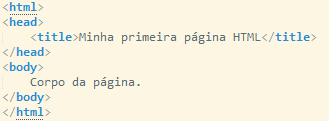
\includegraphics[width=0.75\textwidth]{exhtml.png} %% PARA COLOCAR O ARQUIVO DA IMAGEM NO SHARELATEX, CLIQUE NO ÍCONE QUE PARECE UMA FLECHINHA PARA CIMA (ATUALIZAR), CLIQUE EM UPLOAD E PROCURE A IMAGEM EM SEU COMPUTADOR.
\end{center}
\label{figura1} 
%% LABEL SERVE PARA VOCÊ REFERENCIAR A FIGURA NO MEIO DO TEXTO (VEJA LINHA 330: \ref{figura1}). ASSIM VOCÊ NÃO PERDE A REFERÊNCIA QUANDO MUDA A FIGURA DE LUGAR
\caption{Exemplo de código HTML.}
\end{figure}

\subsubsection{\textit{Cascading Style Sheets} – CSS}

CSS (\textit{Cascading Style Sheets}) – é uma linguagem utilizada para tratamento
visual dos elementos da página \textit{Web} \cite{folle}. Este é, portanto, a tecnologia
responsável por tratar cada elemento da página \textit{Web} visualmente, atribuindo cores e
posições diferentes, dependendo da preferência do programador. Possui sintaxe
simples e assim como as demais tecnologias, utiliza-se de várias palavras em inglês
para especificar os diferentes estilos de propriedades da página.

\begin{figure} [hbt] 
\begin{center}
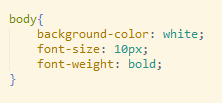
\includegraphics[width=0.75\textwidth]{excss.png}
\end{center}
\label{figura1} 
\caption{Exemplo de código CSS.}
\end{figure}

\subsubsection{\textit{JavaScript e JQuery}}

Segundo \citeonline{folle}, \textit{JavaScript} “é uma linguagem de script executada pelos
navegadores que permite o acesso e manipulação programática de objetos de uma
página \textit{Web}”. Ela possibilita que um campo para digitar uma data seja formatado
automaticamente (com barras), ou que um campo seja desabilitado dinamicamente,
etc. 

\textit{JQuery} é portanto, uma biblioteca de funções prontas de \textit{JavaScript}, que
interagem com o HTML e possibilitam uma melhor experiência ao usuário. Foi lançada
em 2006, no BarCamp, de Nova York, por John Resig e é utilizada por milhares de
sites visitados pelo mundo. Segundo a \citeonline{w3techs}, é a biblioteca JavaScript
mais popular dentre as existentes



\subsection{\textit{Bootstrap}}

\textit{Bootstrap} é o mais popular \textit{framework} de HTML, CSS e \textit{JavaScript} para desenvolvimento de sistemas \textit{Web} de modo responsivo. Esta ferramenta conta com centenas de classes HTML que auxiliam na construção de uma página \textit{Web} \cite{bootstrap}.
Esta ferramenta está presente em cada página do sistema, possibilitando que ele seja acessado de qualquer dispositivo (móvel ou \textit{desktop}). A sua versão estável é a 3.3.7, mas já foi disponibilizada oficialmente a versão 4, versão esta utilizada neste projeto.



\section{Licensa do Software}

O software estará disponível em \url{...} sob a lincensa ???s
% ---
% avaliação
\chapter{Avaliação} \label{ch:avaliacao}

\section{Visão Geral}
\section{Ambiente}
\section{Caracterização dos Participantes}
\section{Tarefas Realizadas}
\section{Resultados}

% ---
% discussao
\chapter{Discussão} \label{ch:discussao}




Com base no levantamento de requisitos, representado pelas histórias de usuário, foi desenvolvido o sistema. Foi feito uma avaliação do sistema sob os critérios de usabilidade, que deve contemplar os seguintes fundamentos: facilidade de uso, facilidade de aprendizado, memorabilidade, produtividade, flexibilidade e satisfação do usuário. Abaixo segue uma tabela com os critérios de usabilidade segundo \citeonline{nogueira}, ao qual sob ele foi formulado o questionário.
O formulário foi criado através do \textit{Google Forms} onde foi possível gerar um questionário que aborde questões que assegurem a IHC (interface humano-computador).

\begin{table}[hbt]
\centering
\begin{tabular}{p{5cm}|p{10cm}}
\hline
\textbf{Critérios de Usabilidade} & \multicolumn{1}{c}{\textbf{Formas de Aferição}}                                                                                                                                                                    \\ \hline
Facilidade de uso                 & Mensurar,a,velocidade,e,a,quantidade,de,erros,durante,a,
execução,de,determinada,tarefa,,que,caso ocorram, devem ser facilmente recuperados; (PREECE, 1994) (NIELSEN, 1993) (ISO 9241-11, 1998) \\ \hline
Facilidade de aprendizado         & Mensurar,o,tempo,e,o,esforço,necessários,para,que,os,
usuários,tenham,um,determinado,padrão,de desempenho; (NIELSEN, 1993) (PREECE, 1994)                                                       \\ \hline
Satisfação do usuário             & Avaliar se o usuário gosta do sistema e sente prazer em trabalhar com ele; (NIELSEN, 1993) (PREECE, 1994) (ISO 9241-11, 1998)                                                                  \\ \hline
Produtividade                     & Mensurar,o,ganho,de,produtividade,do,usuário,ao,
aprender,a,
utilizar,o,sistema,proposto;(NIELSEN, 1993) (ISO 9241-11, 1998)                                                                     \\ \hline
Flexibilidade                     & Avaliar o nível de customização e personalização da interface pelo usuário; (PREECE, 1994)                                                                                                     \\ \hline
Memorabilidade                    & Avaliar,o,nível,de,treinamento,necessário,para,reciclar,
usuários,eventuais,do,sistema. (NIELSEN, 1993)                                                                                         \\ \hline
\end{tabular}
\label{tableNogueira} 
\caption{Critérios de Usabilidade \cite{nogueira}}
\end{table}

Feito a pesquisa através do \textit{Google Forms}, foi obtido os resultados, apresentados a seguir. A pesquisa foi feita com nutricionistas que já faziam o uso do sistema e após o uso, foi solicitado que respondessem ao questionário. O sistema é totalmente gratuito e está disponível no \textit{link}: https://sysnut.herokuapp.com, possuindo apenas limite de acessos mensais, por motivo de seu domínio e hospedagem serem gratuitos.


% ---
% conclusao
\chapter{Conclusão e Trabalhos Futuros}


\section{Contribuições}

O presente trabalho trata de um sistema para nutricionista com o intuito de ajudar a fazer o acompanhamento de dietas com seus pacientes de forma gratuita para ambos, tanto paciente como nutricionista. 
Para solucionar tais problemas, desenvolveu-se um sistema \textit{Web} totalmente gratuito com as
principais funcionalidades elencadas nas histórias de usuário, possibilitando assim
que qualquer usuário (nutricionista ou paciente) pudesse acessá-lo de qualquer
dispositivo com acesso à Internet.

Conforme a avaliação realizada pelos próprios nutricionistas, foi atingido o objetivo do trabalho e com um resultado satisfatório, tendo em vista as respostas obtidas. O nutricionista pode agilizar seu atendimento e se comunicar com o 
paciente através do sistema, melhorando a qualidade do seu serviço. Através do estudo aprofundado das ferramentas utilizadas, foi possível adquirir um conhecimento mais aprofundado sobre o desenvolvimento de sistemas \textit{Web}, além de que foi possível também conhecer a rotina de trabalho do nutricionista e uma vez que estudado o problema, foi possível ajudar a solucioná-lo, possibilitando que se possa reduzir os índices de obesidade existentes no Brasil através da prescrição de dietas que orientem sobre uma alimentação saudável e rica em nutrientes essenciais ao ser humano.


\section{Trabalhos Futuros}
Como trabalhos futuros, planeja-se desenvolver um aplicativo para celulares com sistema operacional Android e iOS,
para que a comunicação entre paciente e nutricionista aconteça de forma mais ágil e também possibilite uma melhor
experiência para ambos.

% ----------------------------------------------------------
% ELEMENTOS PÓS-TEXTUAIS
% ----------------------------------------------------------
\postextual


% ----------------------------------------------------------
% Referências bibliográficas
% ----------------------------------------------------------
\bibliography{references} %% REFERENCIA AO ARQUIVO abntex2-modelo-references.bib

% ----------------------------------------------------------
% Glossário
% ----------------------------------------------------------
%
% Consulte o manual da classe abntex2 para orientações sobre o glossário.
%
%\glossary

% ----------------------------------------------------------
% Apêndices
% ----------------------------------------------------------

% ---
% Inicia os apêndices
% ---

\begin{apendicesenv}
% Imprime uma página indicando o início dos apêndices
\partapendices

\begin{landscape}
% ----------------------------------------------------------
\chapter{\textit{Product BackLog}}
% ----------------------------------------------------------
\begin{table}[h]
\centering
\caption{My caption}
\label{my-label}
\begin{tabular}{|p{0.5cm}|p{2cm}|p{5cm}|p{4cm}|p{2.5cm}|p{3.7cm}|p{2cm}|p{2cm}|}
\hline
\textbf{ID} & \textbf{Ação} & \textbf{Descrição}                                                                                                 & \textbf{Critérios de Aceitação} & \textbf{VN (Valor de Negócio)} & \textbf{Estimativa (Story Points - SP)} & \textbf{ROI (VN/SP)} & \textbf{Sprint} \\ \hline
1                               & Login                             & Sendo um administrador, preciso realizar login no sistema para que possa ter acesso ao sistema como administrador. & Verificar autenticidade; Exibir página do usuário.  & 800                                                & 5                                                           & 160                                      & 1                                   \\ \hline
2                               & Login                             & Sendo um nutricionista, preciso realizar login no sistema para que possa ter acesso ao sistema como nutricionista. & Verificar autenticidade; Exibir página do usuário.  & 1000                                               & 5                                                           & 200                                      & 1                                   \\ \hline
3                               & Cadastro                          & Sendo um nutricionista, preciso cadastrar um novo paciente para que possa fazer sua consulta e seu cardápio.       & Verificar preenchimento dos campos;                 & 3000                                               & 100                                                         & 30                                       & 1                                   \\ \hline
4                               & Cadastro                          & Sendo um nutricionisa, preciso coletar os dados antropométricos do paciente para seja possível realizar a anamnese alimentar com mais precisão. & Verificar preenchimento dos campos;                 & 1000                                               & 40                                                          & 25                                       & 1                                   \\ \hline
5                               & Cadastro                          & Sendo um nutricionista, preciso anexar documentos como laudos médicos para que ateste algum tipo de patologia que o paciente possa ter.         & Verificar preenchimento dos campos;                 & 2000                                               & 50                                                          & 40                                       & 1                                   \\ \hline
6                               & Cadastro                          & Sendo um nutricionista, preciso cadastrar o fator de atividade física do paciente para que o cardápio se adeque a sua rotina.                   & Verificar preenchimento dos campos;                 & 2000                                               & 20                                                          & 100                                      & 1                               	\\ \hline
\end{tabular}
\end{table}

\end{landscape}
\end{apendicesenv}
% ---



\end{document}
